\documentclass[convert={density=300,outext=.png}]{standalone}
\usepackage{tikz}
\usetikzlibrary{shapes,arrows,decorations,decorations.pathmorphing,arrows.meta,patterns,decorations.markings}

\begin{document}
%% Use \usepackage{tikz}
%% Use \usetikzlibrary{shapes,arrows,decorations, decorations.pathmorphing,arrows.meta,patterns}
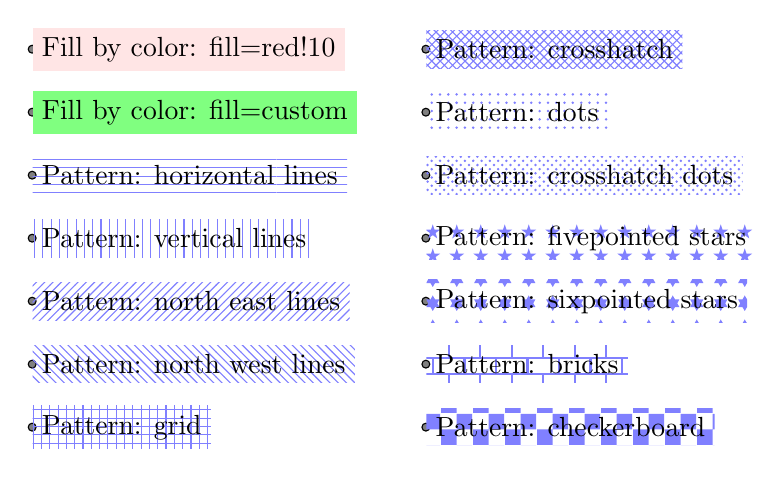
\begin{tikzpicture}[scale=1.0000]
	\tikzstyle{every node}=[scale=1.0000]
	
	\definecolor{a00050b}{RGB}{0,0,0}
	%%Created with tikzpy
	
	\draw [ fill= a00050b!50 ,]  (0.0000,0.0000,0.0000) circle [radius=0.0500];
	\node [ fill= red!10 , ,right]  at (0.0000,0.0000,0.0000)  {Fill by color: fill=red!10};
	\draw [ fill= a00050b!50 ,]  (0.0000,-0.8000,0.0000) circle [radius=0.0500];
	\node [ fill= green!50 , ,right]  at (0.0000,-0.8000,0.0000)  {Fill by color: fill=custom};
	\draw [ fill= a00050b!50 ,]  (0.0000,-1.6000,0.0000) circle [radius=0.0500];
	\node [pattern color=blue!50 ,pattern=horizontal lines ,right]  at (0.0000,-1.6000,0.0000)  {Pattern: horizontal lines};
	\draw [ fill= a00050b!50 ,]  (0.0000,-2.4000,0.0000) circle [radius=0.0500];
	\node [pattern color=blue!50 ,pattern=vertical lines ,right]  at (0.0000,-2.4000,0.0000)  {Pattern: vertical lines};
	\draw [ fill= a00050b!50 ,]  (0.0000,-3.2000,0.0000) circle [radius=0.0500];
	\node [pattern color=blue!50 ,pattern=north east lines ,right]  at (0.0000,-3.2000,0.0000)  {Pattern: north east lines};
	\draw [ fill= a00050b!50 ,]  (0.0000,-4.0000,0.0000) circle [radius=0.0500];
	\node [pattern color=blue!50 ,pattern=north west lines ,right]  at (0.0000,-4.0000,0.0000)  {Pattern: north west lines};
	\draw [ fill= a00050b!50 ,]  (0.0000,-4.8000,0.0000) circle [radius=0.0500];
	\node [pattern color=blue!50 ,pattern=grid ,right]  at (0.0000,-4.8000,0.0000)  {Pattern: grid};
	\draw [ fill= a00050b!50 ,]  (5.0000,0.0000,0.0000) circle [radius=0.0500];
	\node [pattern color=blue!50 ,pattern=crosshatch ,right]  at (5.0000,0.0000,0.0000)  {Pattern: crosshatch};
	\draw [ fill= a00050b!50 ,]  (5.0000,-0.8000,0.0000) circle [radius=0.0500];
	\node [pattern color=blue!50 ,pattern=dots ,right]  at (5.0000,-0.8000,0.0000)  {Pattern: dots};
	\draw [ fill= a00050b!50 ,]  (5.0000,-1.6000,0.0000) circle [radius=0.0500];
	\node [pattern color=blue!50 ,pattern=crosshatch dots ,right]  at (5.0000,-1.6000,0.0000)  {Pattern: crosshatch dots};
	\draw [ fill= a00050b!50 ,]  (5.0000,-2.4000,0.0000) circle [radius=0.0500];
	\node [pattern color=blue!50 ,pattern=fivepointed stars ,right]  at (5.0000,-2.4000,0.0000)  {Pattern: fivepointed stars};
	\draw [ fill= a00050b!50 ,]  (5.0000,-3.2000,0.0000) circle [radius=0.0500];
	\node [pattern color=blue!50 ,pattern=sixpointed stars ,right]  at (5.0000,-3.2000,0.0000)  {Pattern: sixpointed stars};
	\draw [ fill= a00050b!50 ,]  (5.0000,-4.0000,0.0000) circle [radius=0.0500];
	\node [pattern color=blue!50 ,pattern=bricks ,right]  at (5.0000,-4.0000,0.0000)  {Pattern: bricks};
	\draw [ fill= a00050b!50 ,]  (5.0000,-4.8000,0.0000) circle [radius=0.0500];
	\node [pattern color=blue!50 ,pattern=checkerboard ,right]  at (5.0000,-4.8000,0.0000)  {Pattern: checkerboard};

\end{tikzpicture}
\end{document}
